\documentclass[a4paper, 11pt]{article}
\usepackage{comment} % enables the use of multi-line comments (\ifx \fi) 
\usepackage{lipsum} %This package just generates Lorem Ipsum filler text. 
\usepackage{fullpage} % changes the margin
\usepackage{graphicx}
 \usepackage{cite}

\begin{document}
%Header-Make sure you update this information!!!!
\noindent


\part*{Section A}
\section*{Architecture Discussion}

\subsection*{Problem}
The problem is a two class classification problem - occupancy detection based on sensor readings. The recorded sensor data is temperature, humidity, light and carbon dioxide. The features include an additional derived feature, humidity ratio, which was derived from the original recorded variables. Each point in the data set is also timestamped. In \cite{Candanedo2016} the time stamp was used to derive two additional features - week status(WS) and number of seconds from midnight(NSM).
A certain amount of noise is expected in the recorded data so a suitable architecture should have good generalisation. Since data was measured in a controlled environment we expect the range of training variables to roughly match the range of expected data.

\subsection*{Architectures}
There are several neural network architectures suitable for this kind of classification problem - Multilayer perceptron, Radial basis function network and Correlation memory matrix. 
\subsubsection*{Multilayer Perceptron (MLP)}
MLP is a feedforward neural network with multiple neurons composed in multiple layers. All neurons are the same in the case of classification and they compute a weighted sum of inputs and apply an activation function (sigmoid or tanh). There is an input layer, which distributes the inputs, zero or more hidden layers and an output layer. Each layer feeds into the next one. This type of neural network uses and error correcting learning rule and a backpropagation training algorithm. Backpropagation consists of two stages - a forward pass, where outputs are computed and a backward pass where weights are adjusted according to the error in outputs. In the backward pass the output layer weights are adjusted according to the local gradient of the error function and the hidden layer weights are adjusted according to the local gradients of the nodes in the subsequent layer. 
\subsubsection*{MLP Advantages and disadvantages}
The multilayer perceptron is suiatable for nonlinearly seperable classification problems. Once a good aproximate solution is found generalisation can be easyly improved by adjusting the stopping criteria of the training algorithm or using regularisation. MLP is a global approximator (because it split's the entire pattern space using lines), which can be an advantage if dataset we have doesn't describe the full range of expected data. \\ 
Determining the number of hidden layers and number of neurons in each layer may require a lot of experimentation. The training algorithm uses local gradients and can often get stuck in a local minimum of the error function. 


%MLP is a feedforward, multilayer architecture consisting of one input layer, one output layer and hidden layers. The input layer just passes on the inputs. Each neuron in the hidden layers computes a weighted sum of inputs, applies a transfer function and passes it's output to each neuron in the next layer. Each layer feeds into the next and the output layer produces the outputs. The MLP uses an error correction learning rule, where it minimises an error function defined by the difference of it's output and the desired output (typically the error function is mean squared error). In order to minimise the error function, it needs to be continuous, therefore the transfer function of each neuron is either a hyperbolic tangent function or a sigmoid function. The training algorithm for MLP is backpropagation. It consists of a forward pass, where the network computes it's output and a backward pass, where the weights are adjusted. Weight changes at each layer are computed based on the local gradient of the next layer. The MLP classifies patterns by partitioning the feature space into regions. It can be used to solve linearly inseparable classification problems, as each layer computes a non-linear transformation of the outputs of the previouse one.
\subsubsection*{Radial Basis Function Network (RBF)}
RBF is a feedforward network, consisting of single hidden layer and an input and output layer. Input layer just distributes inputs to the hidden layer. Each neuron in the hidden layer computes a radially symmetric basis activation function (typically a Gaussian) from the inputs. The output layer neurons compute a weighted sum of the outputs of the hidden layer. Each neuron in the hidden layer has two associated parameters - a point in the feature space, which is called a center, and a spread. It computes it's response to a given input based on the euclidean distance between the data point and it's center. Training is typically done in two stages - center selection and weight estimation, where wighgts can be cimputed in a single matrix vector calculation. RBFs can also be trained in a supervised manner (like MLP) or by selecting centers at each data point and using regularisation, but these aproaches are much slower.
\subsubsection*{RBF Advantages and Disadvantages}
There is only one hidden layer so we only need to experiment with it's size. When using unsupervised center selection, weights can be computed in a single calculation. There are much less architecture parameters that can be varied when searching for an  architecture compared to the MLP. The RBF is a local aproximator, which is an advantage when we expect new data to be in a similar range to the training data or when abnormal inputs need to be ignored. \\
It is difficult to determine center locations. When data isn't clustered might need a very large hidden layer.  Supervised center selection and regularisation training approaches are very slow. 

\subsubsection*{Correlation Matrix Memory(CMM)}
CMMs are single layer neural networks, which use the Hebbian learning rule. They consist of a single weight matrix which stores correlations between input and output patterns. Learning is done by computing the outer product of the input and output and adding it to the outer products of all other patterns to form the weight matrix. Recall of a stored pattern is done by multiplying the weight matrix and the input. For efficiency these networks usually have binary inputs and weights. In order to use a CMM as a classifier the output needs to be threasholded, so the highest output value is set to 1 and represents the class, or some kind of postprocessing needs to be done such as the one used in \cite{Zhou1998}.  
\subsubsection*{CMM advantages and disadvantages}
A hardware implementation of CMM can be very fast. Training and recall are both very fast operations. \\
A CMM can store a limited number of pattern associations after which new associations become diluted. Real valued data needs to be encoded using a binning algorithm. Best performance requires input patterns to follow a uniform distribution. Good classification might require additional post processing (e.g. k nearest neighbours).

\subsubsection*{Advantages/Disadvantages}
%The Perceptron is a very simple and quick to train network consisting of a single neuron. However it can easily be ruled out because of it's inability to classify linearly inseperable problems. From figure \ref{fig:plotmatrix} we can clearly see that our data is linearly inseperable when looking at the relation between Hummidity and CO2 for example. 
%The MLP is suatable for solving non-linearly seperable problems. It's iterative training process can be slow depending on the error function minimisation method used, however it is very customisable. Once a good aproximate solution is found generalisation can be easyly improved by adjusting the stopping criteria of the training or employing regularisation. Choosing the right size of the network might require a lot of trial and error. The MLP is global aproximator, which might be an advantage when we could expect new data to be significantly different from training data.
%The RBF has a single hidden layer. Training can be very slow when using supervised selection of centers or regularisation. There are much less architecture parameters that can be varied when searching for a suitable architecture compared to the MLP. The RBF is a local aproximator, which is an advantage when we expect new data to be in a similar range to the training data and can also be used for detecting abnormal inputs. 

%\subsection*{Data exploration}
%All features - Temperature, Humidity, Light, CO2, Humidity Ratio are real valued. In figure \ref{fig:plotmatrix} the MATLAB $gplotmatrix$ function is used to plot all variables against each other and create histograms of each variable along the diagonal and class are color coded.  

\subsubsection*{Choice of network architecture}
Comparing the three architectures stated above we choose an RBF network architecture. Compared to the MLP the RBF has a simpler training process. Furthermore, using our knowledge of the problem we can see that the data we have should more or less be like the expected data after training. Because of this an RBF would be more suitable as a local classifier rather than an MLP.
The CMM is superior in terms of speed, and would be a very suitable choice for a real time application. However it would require further domain knowledge of the data in order to decide on encoding of inputs. The CMM's capacity limitations might mean we would need a very large weight matrix. 

\begin{figure}[h]
  \caption{Scatter plot matrix}
  \centering
    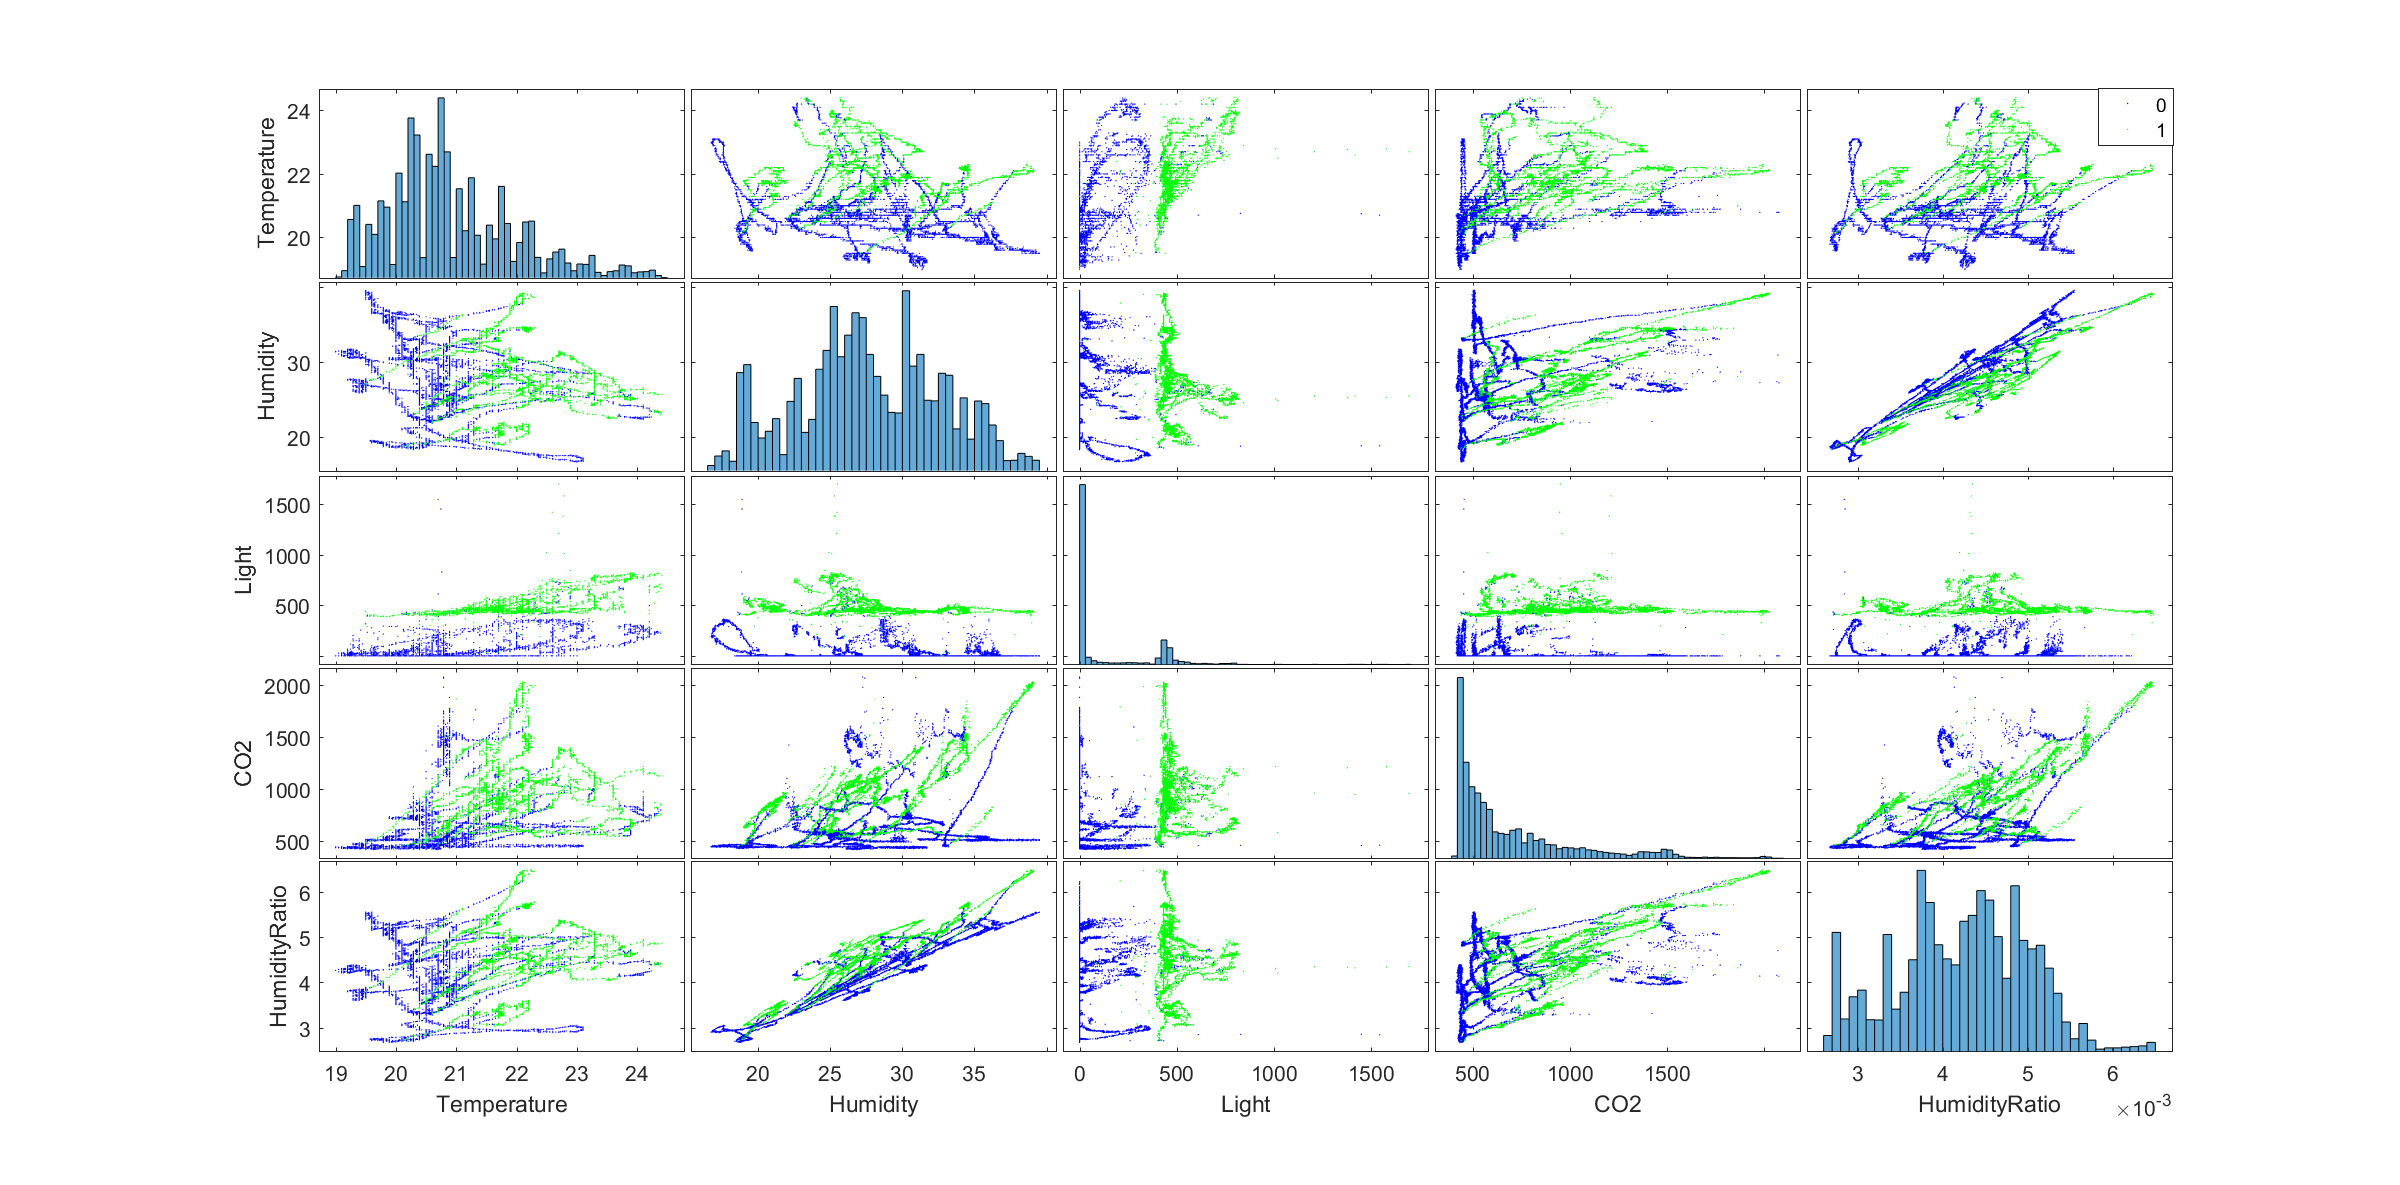
\includegraphics[width=1\textwidth]{Plotmatrix.png}
    \label{fig:plotmatrix}
\end{figure}
\subsection*{Experiments}





\section*{Creation and Application}
\lipsum[2]

\subsection*{Data}
\lipsum[3]

\subsection*{Network}
\lipsum[4]

\subsection*{Training}
\lipsum[4]

\subsection*{Evaluation}
\lipsum[4]

\subsection*{Results}
\lipsum[4]
% to comment sections out, use the command \ifx and \fi. Use this technique when writing your pre lab. For example, to comment something out I would do:
%  \ifx
%	\begin{itemize}
%		\item item1
%		\item item2
%	\end{itemize}	
%  \fi





\part*{Section B}




\bibliographystyle{plain}
\bibliography{science}
\end{document}
